%% Include the picture as follows: \
% \begingroup
% \tikzset{every picture/.style={scale=1,radius=0.05,line width=0.4}}%
% \input{tikz/[filename].tex}%
% \endgroup
%
%% Want to add a label? Use node[<position>]{label},
%% where <position> is one of: below / above / left / right
% \fill (0,0) circle node[below]{$p_1$};
%% Want to give the point a different color?
% \fill[red] (0,0) circle;
%
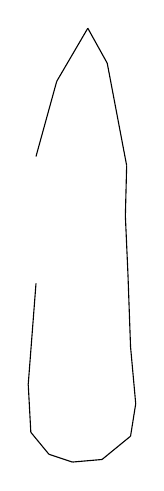
\begin{tikzpicture}
\draw (4.5033,8.8454) -- (4.7500,8.4013);
\draw (4.1086,8.1711) -- (4.5033,8.8454);
\draw (4.7500,8.4013) -- (4.9967,7.1020);
\draw (4.9803,6.4605) -- (4.9967,7.1020);
\draw (5.0461,4.7993) -- (5.0132,5.7204);
\draw (4.9803,6.4605) -- (5.0132,5.7204);
\draw (5.0461,4.7993) -- (5.1118,4.0757);
\draw (5.0461,3.6645) -- (4.6842,3.3684);
\draw (5.1118,4.0757) -- (5.0461,3.6645);
\draw (4.3059,3.3355) -- (4.0099,3.4342);
\draw (4.6842,3.3684) -- (4.3059,3.3355);
\draw (4.0099,3.4342) -- (3.7796,3.7138);
\draw (3.7796,3.7138) -- (3.7467,4.3224);
\draw (3.8454,5.6053) -- (3.7467,4.3224);
\draw (3.8454,7.2171) -- (4.1086,8.1711);
\fill (4.5033,8.8454) circle;
\fill (4.7500,8.4013) circle;
\fill (4.9967,7.1020) circle;
\fill (4.9803,6.4605) circle;
\fill (5.0132,5.7204) circle;
\fill (5.0461,4.7993) circle;
\fill (5.1118,4.0757) circle;
\fill (5.0461,3.6645) circle;
\fill (4.6842,3.3684) circle;
\fill (4.3059,3.3355) circle;
\fill (4.0099,3.4342) circle;
\fill (3.7796,3.7138) circle;
\fill (3.7467,4.3224) circle;
\fill (3.8454,5.6053) circle;
\fill (3.8454,7.2171) circle;
\fill (4.1086,8.1711) circle;
\end{tikzpicture}
